\section{Path Planning using Reinforcement Learning}

\subsection{Environment}

The environment used for model training was based on the Fetch Reach environment made available by Gymnasium Robotics (https://robotics.farama.org/envs/fetch/reach/). In this environment, the task was to make the manipulator move the end-effector to a random 3D position above a table in front of the robot, as show in \autoref{fig:fetch_reach_env}. The robot in this simulation has 7-DoF and is controlled by small displacements of the gripper in cartesian coordinates, with Mujoco being responsible for the inverse kinematics computation.

\begin{figure}[H]%[ht]
    \centerline{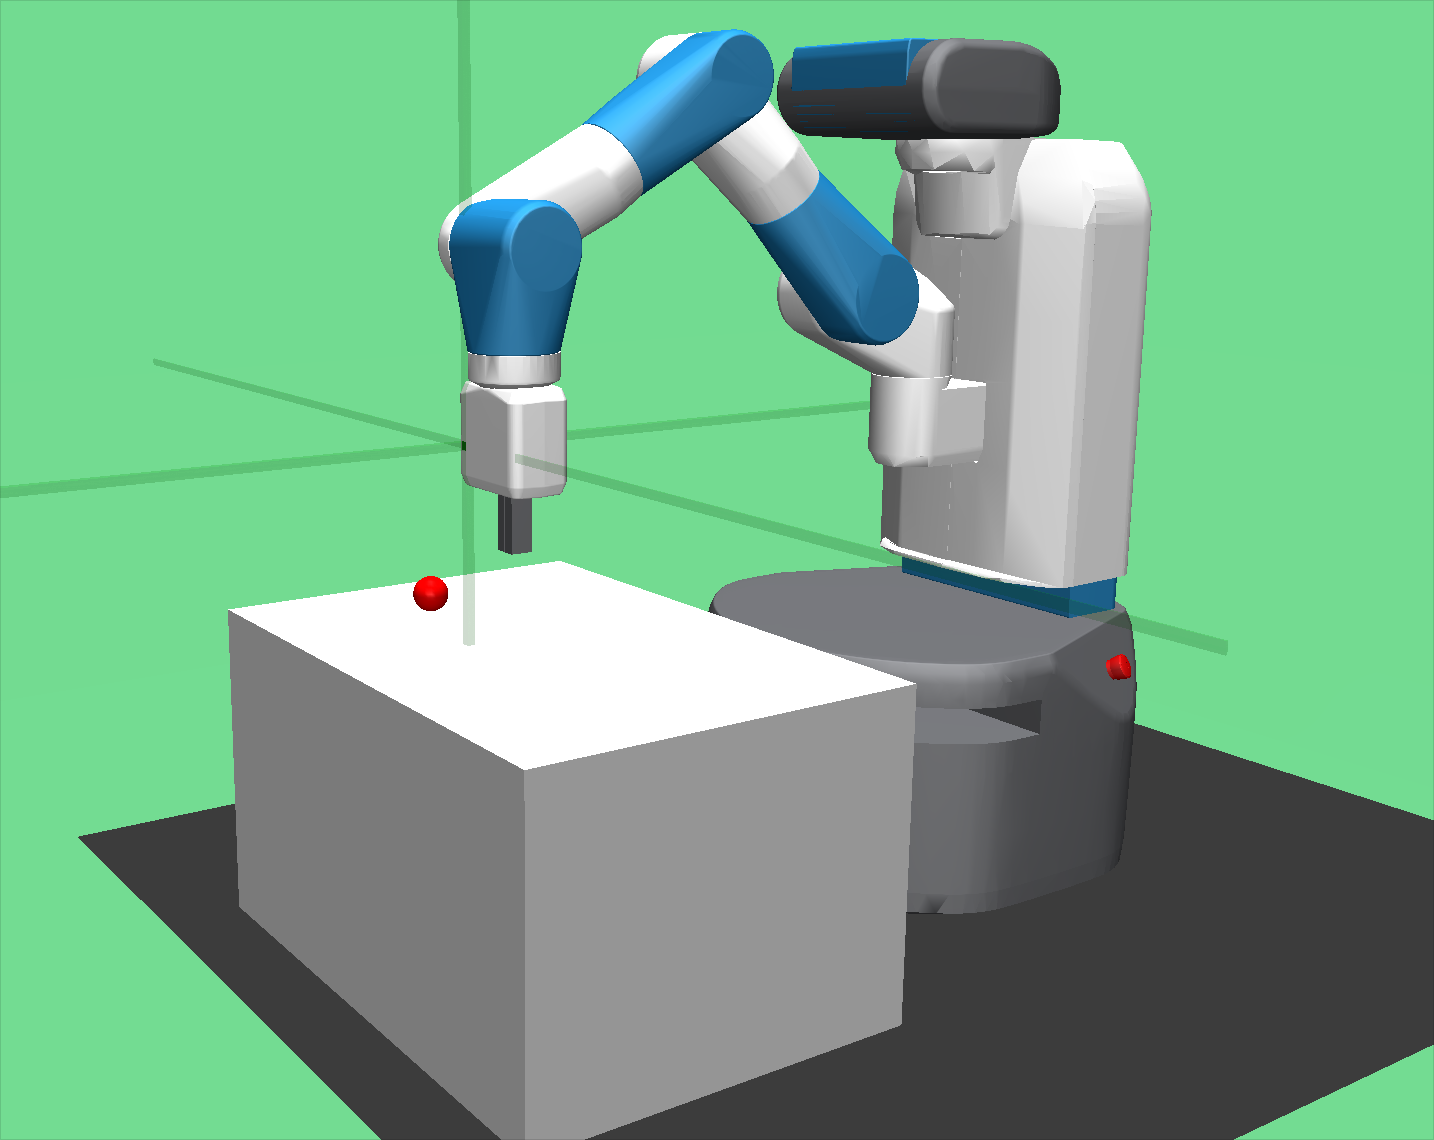
\includegraphics[width=0.7\textwidth]{figs/fetch_reach.png}}
    \caption[Fetch Reach Environment]{Fetch Reach Environment}
    \label{fig:fetch_reach_env}
\end{figure}

The Fetch Reach environment served as a starting point for this research but ended up being mostly rewritten to not only resemble the available collaborative cell but also allow for direct joint control instead of the previous cartesian displacements. The final environment, now named Larcc, can be seen in \autoref{fig:larcc_env} which now includes a UR10e robot model with a Robotiq 2F-140 gripper just like in the real collaborative cell. \textcolor{red}{(should probably refer the sources of the models around here)} The models used were deemed acceptable given that the difference between the end-effector position in ROS and in the simulator differ by less than 1mm for the same joint positions. In this environment, the goal is to move the end-effector to a target position and orientation which are both represented by 3D axes in the simulator. As the actions affect the joints directly, a model trained is this environment ends up replacing the inverse or differential kinematics.

\begin{figure}[H]%[ht]
    \centerline{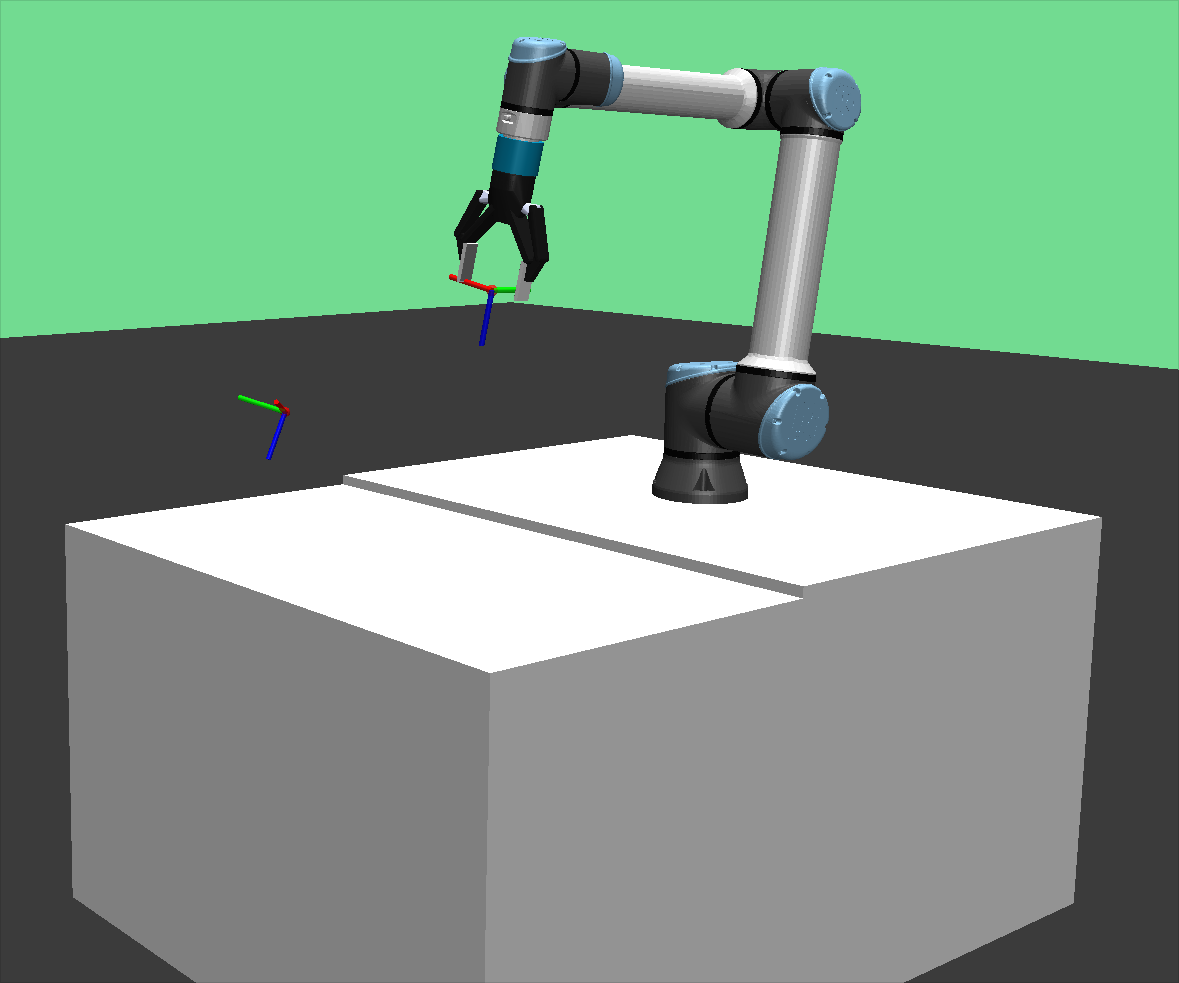
\includegraphics[width=0.7\textwidth]{figs/larcc_env.png}}
    \caption[Larcc Environment]{Larcc Environment}
    \label{fig:larcc_env}
\end{figure}

\subsubsection{Starting State}

To set up a new episode during training, the robot state and the goal position and orientation in the environment are reset.

For the goal, the position is sampled from a uniform distribution corresponding to the volume \SI{10}{\cm} to \SI{60}{\cm} above the table in front of the robot. The orientation is sampled from a uniform distribution in RPY format and then converted to quaternions. The orientation is then validated to check if it is facing mostly forward and downwards, which is the orientation that the gripper should have to pick up an object. If the orientation is not valid, a new one is sampled until a valid one is found.

For the starting state of the robot there are two possibilities: it can start in the fixed position shown in \autoref{fig:larcc_env} or in a random position. The random position is obtained by sampling the joint positions from a uniform distribution in the $[-\pi, \pi]$ interval, which is the same interval used for the joint limits in the UR10e robot. However, given that a fully random starting position can make the task too difficult, the end-effector position and orientation from the random starting position is validated with the same constraints as the goal position and a new starting position is sampled until a valid one is found.

\subsubsection{Observation Space}

The observation space in this environment follows the structure commonly used Gymnasium environments being a dictionary with 3 keys:

\begin{itemize}
    \item $observation$: consists of the positions of the 6 joints; given that they were limited to the $[-\pi, \pi]$ interval, they were normalized by a division by $\pi$;
    \item $achieved\_goal$: current position and orientation of the end-effector; the position was normalized by subtracting the position of the robot base link in the environment and then dividing by the arm's range, and the orientation was kept because it is defined with quaternions which are already in the $[-1, 1]$ interval;
    \item $desired\_goal$: position and orientation of the goal; normalized in the same way as the achived\_goal above.
\end{itemize}

\subsubsection{Action Space}

The action space represents the displacements in all joints for a single timestep. These displacements are also normalized which means that the final action applied to the environment is the result of the action output given by a model which is in the $[-1, 1]$ range multiplied by the maximum displacements of the joints. The first two joints associated with the shoulder can move at most 0.8 radians per timestep while the other four joints associated with the elbow and the wrist can move at most 1.2 radians per timestep, representing the different maximum velocities on the UR10e robot joints (https://www.universal-robots.com/products/ur10-robot/).

\subsubsection{Rewards}

The used environment has dense rewards so as to give the agent frequent and consistent feedback about its actions. This means that in every timestep the reward will increase if the the end-effector is closer to the goal and decrease otherwise, helping the model learn which actions lead to a successful episode. The reward in each timestep is obtained from the following rewards:

\begin{itemize}
    \item $position$: $1-distance(goal\_pos, end$-$effector\_pos)$ if distance lower than 2 otherwise $-1$ so that it is normalized;
    \item $orientation$: $max(innerproduct(goal\_quaternion, end$-$effector\_quaternion), innerproduct(-goal\_quaternion, end$-$effector\_quaternion)$;
    \item $bonus$: $1$ if goal has been reached else $0$; the goal is considered reached if both the other rewards are above $0.98$.
\end{itemize}

These rewards affect the final timestep reward with different weights, but the sum of the weights is always equal to $1$ keeping the final reward in the $[-1, 1]$ range.

\subsection{Soft Actor-Critic (SAC) Model}

\textcolor{blue}{The tests in the described environment were executed using the Soft Actor-Critic (SAC) algorithm. SAC is an off-policy model-free reinforcement learning algorithm that is based on the maximum entropy reinforcement learning framework. This framework allows the agent to learn a policy that maximizes the expected reward while also maximizing the entropy of the policy. This means that the agent will not only try to maximize the reward but also to explore the environment as much as possible. The entropy term in the loss function is weighted by a temperature parameter $\alpha$ which is learned by the model.}

\subsection{Results}

A SAC model was trained on the developed environment with a fixed initial robot state and with a $0.5$ weight on the position reward and a $0.25$ weight on the orientation and on the bonus reward. The model was trained with early stopping configured to evaluate the model every $500$ episodes and stop training if the evaluation average reward does not increase for $20$ evaluations. \autoref{fig:actor_loss} and \autoref{fig:critic_loss} show the evolution of the actor and critic loss during training.

\begin{figure}[H]%[ht]
    \centering
    {\fontsize{8}{11}\selectfont\includesvg[width=\textwidth]{figs/actor_loss.svg}}
    \caption{SAC Actor Loss during Training}
    \label{fig:actor_loss}
\end{figure}

\begin{figure}[H]%[ht]
    \centering
    {\fontsize{8}{11}\selectfont\includesvg[width=\textwidth]{figs/critic_loss.svg}}
    \caption{SAC Critic Loss during Training}
    \label{fig:critic_loss}
\end{figure}

\autoref{fig:entropy_coefficient} shows the evolution of the entropy coefficient during training. A higher entropy coefficient indicates increased exploration of the environment by the model. Considering the reward components in \autoref{fig:reward_components}, the entropy coefficient initially descreases as the model learns to maximize the position and orientation reward but then increases again as the model tries to maximize the bonus reward. 

\begin{figure}[H]%[ht]
    \centering
    {\fontsize{8}{11}\selectfont\includesvg[width=\textwidth]{figs/entropy_coefficient.svg}}
    \caption{SAC Entropy Coefficient during Training}
    \label{fig:entropy_coefficient}
\end{figure}

\begin{figure}[H]%[ht]
    \centering
    {\fontsize{8}{11}\selectfont\includesvg[width=\textwidth]{figs/reward_components.svg}}
    \caption{SAC Episode Reward Components Mean (Max 50) during Training}
    \label{fig:reward_components}
\end{figure}

\autoref{fig:reward} and \autoref{fig:success_rate} show the evolution of the episode reward mean and the success rate during training. The success rate is calculated as the percentage of episodes where the episode is successful which also corresponds to the episodes where there is bonus reward. The success rate is a good indicator of how well the model is learning to reach the goal. Considering that the maximum reward in a single episode is $50$, the model was able to reach a reward close to the maximum. Additionally, the fact that the validation reward is higher than the training reward is expected given that the in the trainig episodes the model attempts to explore the environment according to its entropy while in the validation episodes the model takes the best actions according to its learned policy.

\begin{figure}[H]%[ht]
    \centering
    {\fontsize{8}{11}\selectfont\includesvg[width=\textwidth]{figs/reward.svg}}
    \caption{SAC Episode Reward Mean (Max 50) during Training}
    \label{fig:reward}
\end{figure}

\begin{figure}[H]%[ht]
    \centering
    {\fontsize{8}{11}\selectfont\includesvg[width=\textwidth]{figs/success_rate.svg}}
    \caption{SAC Success Rate during Training}
    \label{fig:success_rate}
\end{figure}

\autoref{tab:sac_results} shows the results when the best model was saved.

\begin{table}[ht] 
\centering
\caption{SAC Results when the Best Model was Saved}
\label{tab:sac_results}
\begin{tabular}{ccc}
\toprule
\multirow{2}{0.25\textwidth}{\centering Training Episodes} & \multirow{2}{0.25\textwidth}{\centering Training Episode Reward Mean} & \multirow{2}{0.25\textwidth}{\centering Validation Episode Reward Mean} \\
& & \\
\midrule
53500 & 42.9 & 45.3\\
\bottomrule
\end{tabular}
\end{table}

